Here we detail the underlying mechanisms that lead to the differences in
distributed performance outcomes between \texttt{ArrayChannels.jl} and
\texttt{Distributed.jl}, as well as provide a brief introduction to our
evaluation benchmarks. The mechanisms that we refer to involve access
locality for processer caches, as well as a discussion on the various
modes of message passing in distributed envirenments.

We discuss our evaluation benchmarks, including a subset of the Intel
Parallel Research Kernels.

\subsection{Access Locality}
\label{sec:access-locality}

Access locality \cite{patterns} describes the patterns at which program
memory is accessed. These patterns are said to either be temporal or
spatial. Temporal locality refers to the proximity of multiple
consecutive accesses to the same memory region, while spatial locality
refers to the proximity of relevant data entries to one another in main
memory.

\subsubsection{Temporal Locality}
\label{sec:temporal-locality}

Essentially, temporal locality in part determines the maximum amount of
time for which program data may remain at readily-accessible regions of
the memory hierarchy. When a greater proportion of the computational
effor can be performed on data currently residing in processor cache,
the total effect of memory latency is mitigated. Alternatively, poor
temporal locality can lead to \emph{cache misses}, scenarios where cache
is prematurely flushed, and program data must be refetched prior to use,
leading to more memory latency. Intuitively, programmers will wish to
ensure when possible that data structures under perpetual use within the
program remain within processor cache, so that all modifications to this
data may incur less overhead. In section~\ref{sec:arraychannels}, we
discuss how in a message-passing context, how retaining a single message
buffer for repeat communication events can lead to improved parallel
performance.

\subsection{Spatial Locality}
\label{sec:spatial-locality}

Spatial locality is a measure the efficiency of cache prefetching in
retrieving as much program data as possible. To improve spatial locality
usually means rearranging or reshaping program data to increase the
proportion of cache lines that are relevant to the task at hand. In the
case of array manipulation, the contiguous property of the underlying
memory ensures a high degree of spatial locality, however programmers
must still consider the effects of striding on multidimensional arrays.

\subsection{Message Passing Models}
\label{sec:message-passing}

Message passing provides a mode for both synchronisation and the
communication of data between processes in a parallel computation. This
methodology is particularly useful when there is no notion of shared
memory between processes, as in the case of distributed computing. Julia
implements message passing through its \texttt{Distributed.jl} module in
the standard library. The two main primatives available to the user are
remote calls, as well as \texttt{Future} objects. Processes may message
one another by means of a remote procedure call, whereby parameters to
the remote call and other captured variables are communicated to the
recipient process. A \texttt{Future} fulfills the synchronising role of
a remote call, encapsulating the completion state of function in
execution at another process.

A combination of these two primatives form the \texttt{RemoteChannel},
which is a sort of handle to a \texttt{Channel} construct appearing at
another worker process. While a \texttt{RemoteChannel} may provide both
synchronous and asynchronous communication, both forms will invoke an
eager communication model. We provide a description of two different
modes of point-to-point message passing in play in both
\texttt{Distributed.jl} and \texttt{ArrayChannels.jl}.

\subsubsection{Eager Communication}
\label{sec:eager}

In eager message passing, processes will immediately attempt to send
messages \cite{illinois, ompi}, without needing to first wait for the
approval of the recipient process. Eager communication permits expensive
communication operations to be initiated prior to the arrival of a
`ready to receive' notification. In various MPI implementations such as
OpenMPI, this is facilitated by the short message protocol, which causes
the message to be copied to the output buffer when specified by the
receive notification. In the case of Julia, this memory copy is not
required, as each message that arrives will have a new output buffer
allocated for immediate use.

\begin{figure}[htb]
  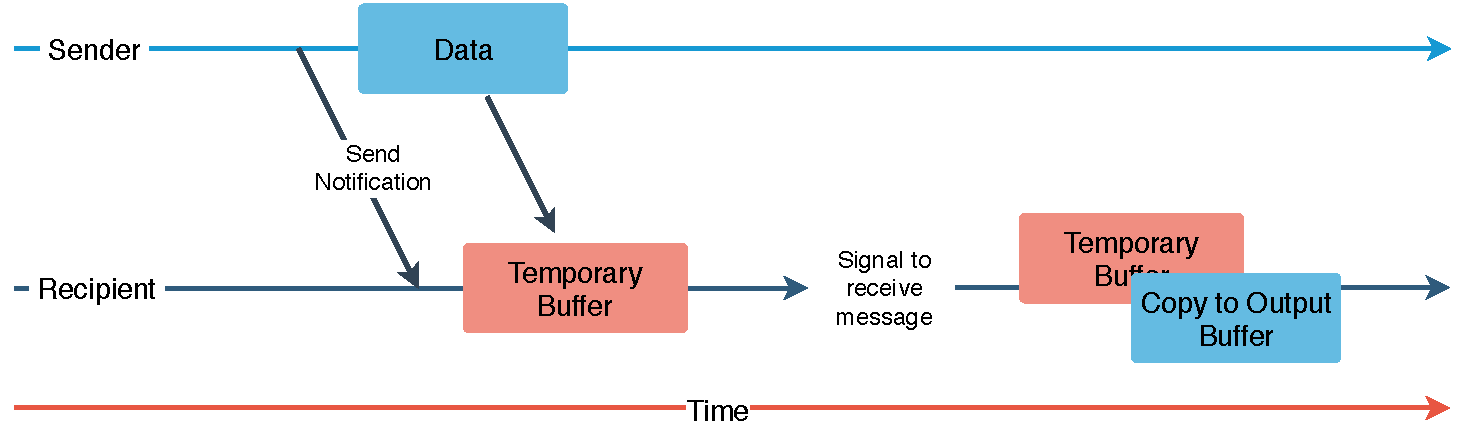
\includegraphics[width=\linewidth]{figs/Eager.pdf}
  \caption{The eager communication model}
  \label{fig:eager}
\end{figure}

The \texttt{Distributed.jl} framework causes messages to be sent in an
eager manner, even on synchronous channel constructs. While access to a
\texttt{RemoteChannel} may be synchronised, any attempt to \texttt{put!}
(or initiate sending) a reference type will fully transfer the
referenced data, but only depositing the reference pointer in the
recipient's channel reference when it is signaled as able to do so. In
section~\ref{sec:transpose-results}, we discuss how eager message
passing can provide performance advantages under pathological examples.

\subsubsection{Rendezvous Communication}
\label{sec:rendezvous}

Rendezvous communication involves both sender and recipient
synchronising over either mutual acknowledgement of messaging, or on the
completion of the data transfer \cite{illinois, ompi}. In the rendezvous
mode, data will not begin to be transfered until both sender and
receiver have each confirmed by means of a handshake the intent to
begin. While rendezvous communication requires that message transfer
occur at a particular time (namely, following a successful handshake),
the receiving process may offer in their intention to receive a prefered
buffer which may be written to directly after synchronisation. In this
way, rendezvous message passing may be used to avoid an extraneous
memory copy, at the cost of requiring additional synchronisation.

\begin{figure}[htb]
  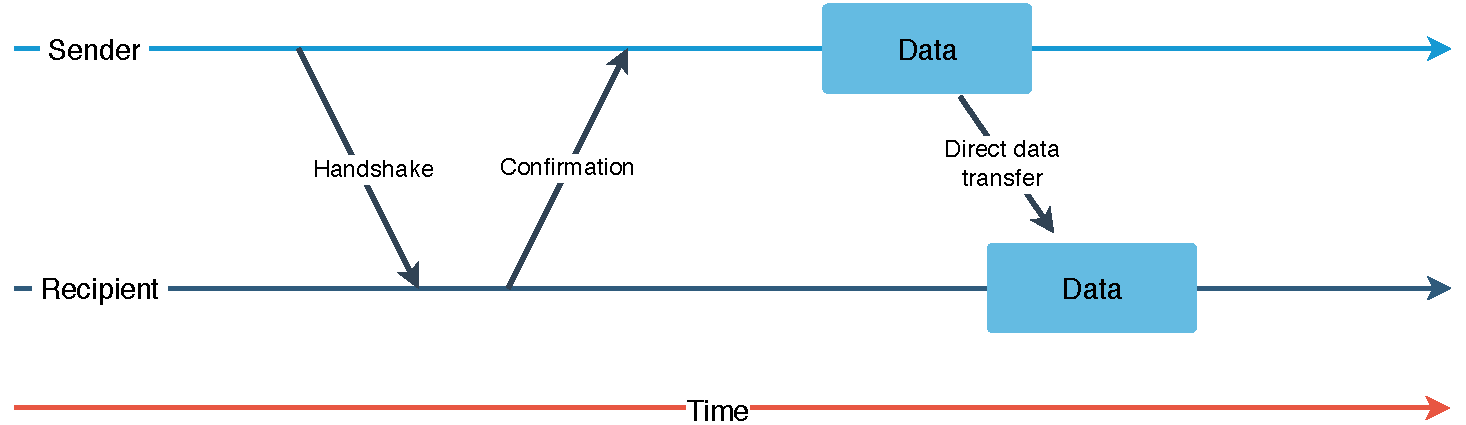
\includegraphics[width=\linewidth]{figs/Rendezvous.pdf}
  \caption{The rendezvous communication model}
  \label{fig:rendezvous}
\end{figure}

An \texttt{ArrayChannel} construct will require rendezvous message
passing to ensure that the same output buffer is used for each
successive communication instance. We discuss how the differences
between these two modes affect the behaviour of the
\texttt{ArrayChannels.jl} library in~\ref{sec:arraychannels}.

\subsection{Evaluation Techniques}
\label{sec:eval}

To evaluate differing performance outcomes between
\texttt{Distributed.jl} and \texttt{ArrayChannels.jl} communciation
nodes, we provide performance comparison on a series of benchmarks. For
an analysis of maximum obtainable data-transfer rate, we provide the
results of a two-process ping-pong benchmark. As a projection of
performance outcomes on more realistic usecases, we compare performance
readings on a subset of the Intel Parallel Research Kernels, providing
readings for a variety of core-counts to indicate the effect of
\texttt{ArrayChannels.jl} communciation primatives on scalability. Our
scalability results are given in terms of weak-scaling, whereby problem
size increases roughly linearly with core-count, to enable each parallel
entity to operate on the same amount of local data.

\subsubsection{Intel Parallel Research Kernels}
\label{sec:intel-prk}

The Intel PRK\textasciitilde{}\cite{Wijngaart} are a series of HPC
kernels that serve to predict the performance of parallel environments
and frameworks for realistic computation tasks.

We provide performance measurements on three of these kernels, namely
Reduce, Transpose and Stencil, due to their emphasis on array computing
which is a strength of the Julia language. Moreover, these kernels
represent real data-parallelism workloads, which are commonplace in the
numerical computing applications of the language.

\subsubsection{Reduce}

The reduce kernel reduces a series of large vectors by accumulating
their vector sum into an output vector at each iteration. For each
additional core provided to the kernel, two vectors of equal size are
provided so as to provide each core with some local computation.

\begin{figure}[htb]
  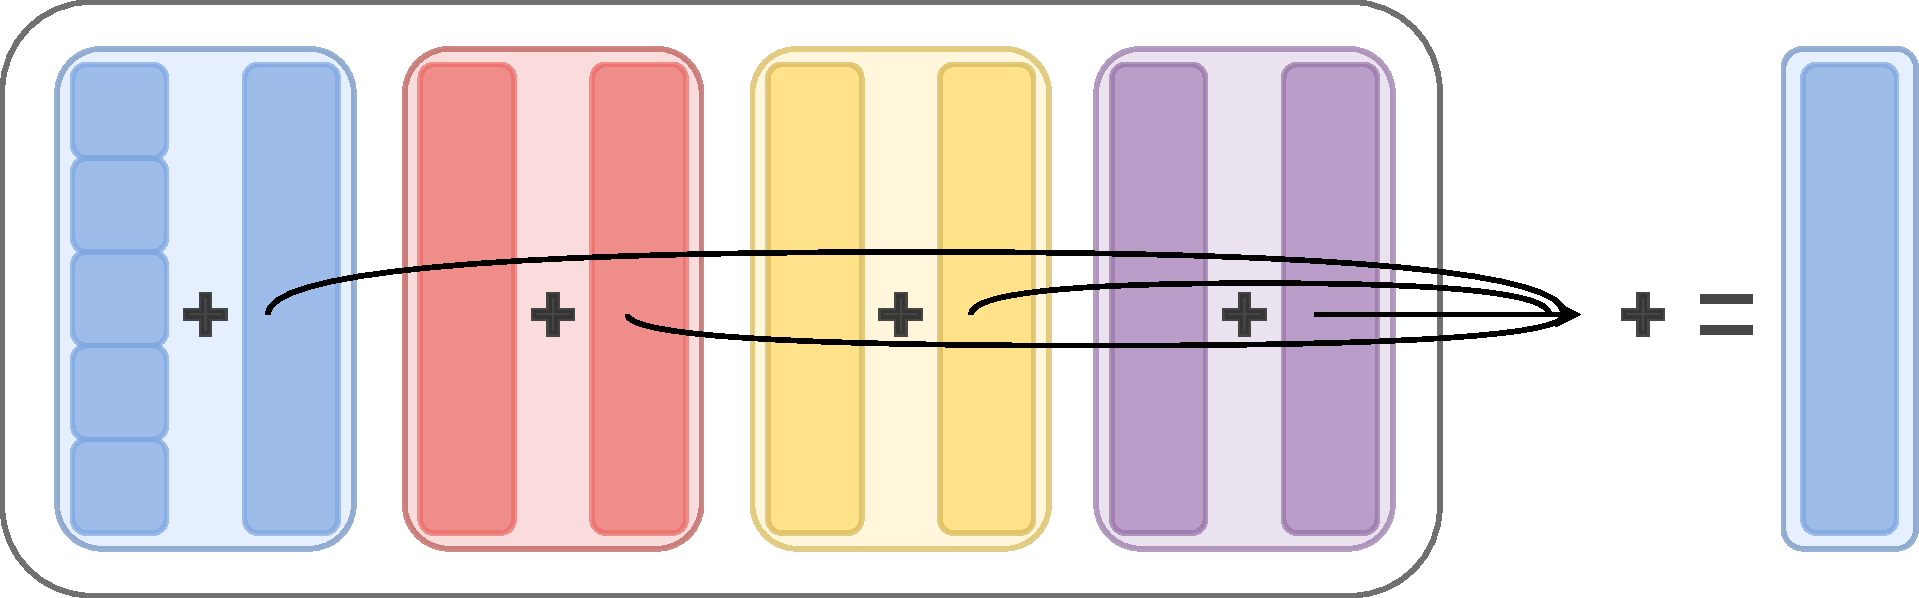
\includegraphics[width=\linewidth]{figs/Reduce.pdf}
  \caption{Reduce kernel}
  \label{fig:reduce-diagram}
\end{figure}

In a distributed context, this is accomplished by allocating two large
vectors at each locale, computing the local sum and then performing a
distributed reduction on the resultant vector. In MPI, this is
facilitated by directly by the \texttt{MPI\_Reduce} directive, which
causes the MPI runtime to conduct the parallel reduction with a single
destination rank using whichever topology it deems most suitable. As the
MPI Reduce implmentation performs its work in place, our equivalent
implementations in Julia attempt to duplicate this behaviour by
implementing the tree topology using point-to-point communication. In
section~\ref{sec:reduce} we comment on the utility of language
directives for directly addressing parallelism patterns.

\subsubsection{Transpose}
\label{sec:transpose-kernel}

The transpose kernel will at each iteration transform the memory
representation of a dense matrix so that columns are stored in the row
format and vice versa. In a distributed context, where the matrix is
fragmented among different locales, the transpose of a pair of indices
may belong to a different locale, and as such data communication is
required. In practise, the matrices are distributed into `column
blocks', with one column block given to each process. Figure~\ref{fig:transpose-diagram} demonstrates how off-diagonal regions of
column blocks must be communicated with other processes at each
iteration.

\begin{figure}[htb]
  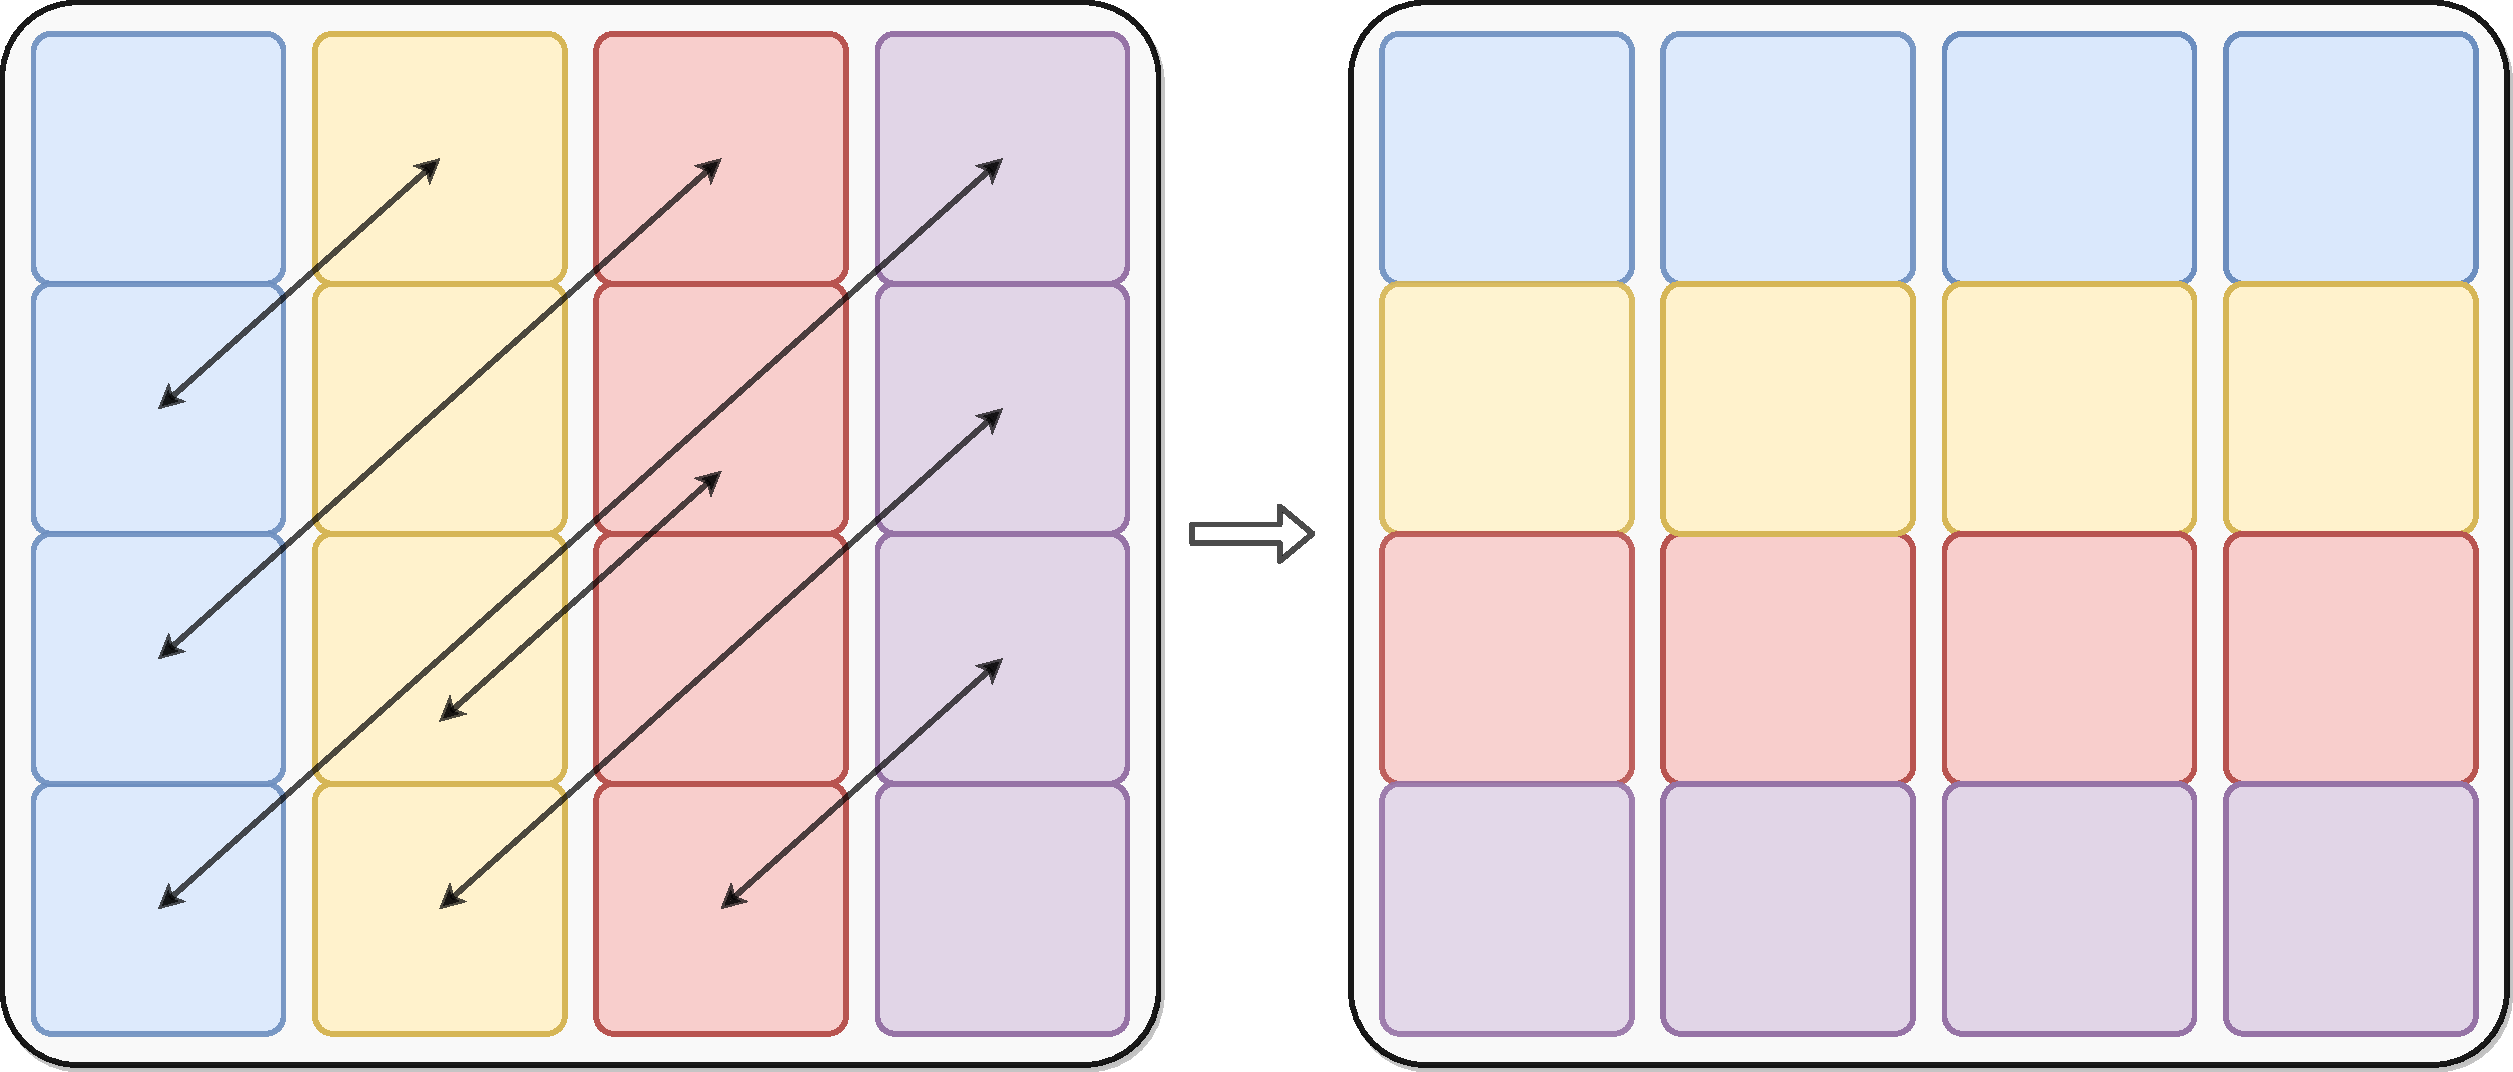
\includegraphics[width=\linewidth]{figs/Transpose.pdf}
  \caption{Distributed transpose kernel}
  \label{fig:transpose-diagram}
\end{figure}

At each iteration, the total amount of data that must be communicated
increases quadratically with the order of the matrix, and each worker
must communicate with every other worker. This kernel provides an
intense stress on the efficiency of the communication model, while
providing minimal arithmetic intensity.

\subsubsection{Stencil}

The stencil kernel involves repeatedly applying a pointwise operator to
each element of a dense matrix, where the point-wise operator depends on
the value of neighbouring datapoints. For a distributed context, this
kernel may be parallelised by decomposing the source matrix into square
blocks and distributing each block to a different worker process.
Applying the stencil operator to indices that border the divisions will
require the acquisition of data from neighbouring processes, as depicted
in figure~\ref{fig:stencil-diagram}.

\begin{figure}[htb]
  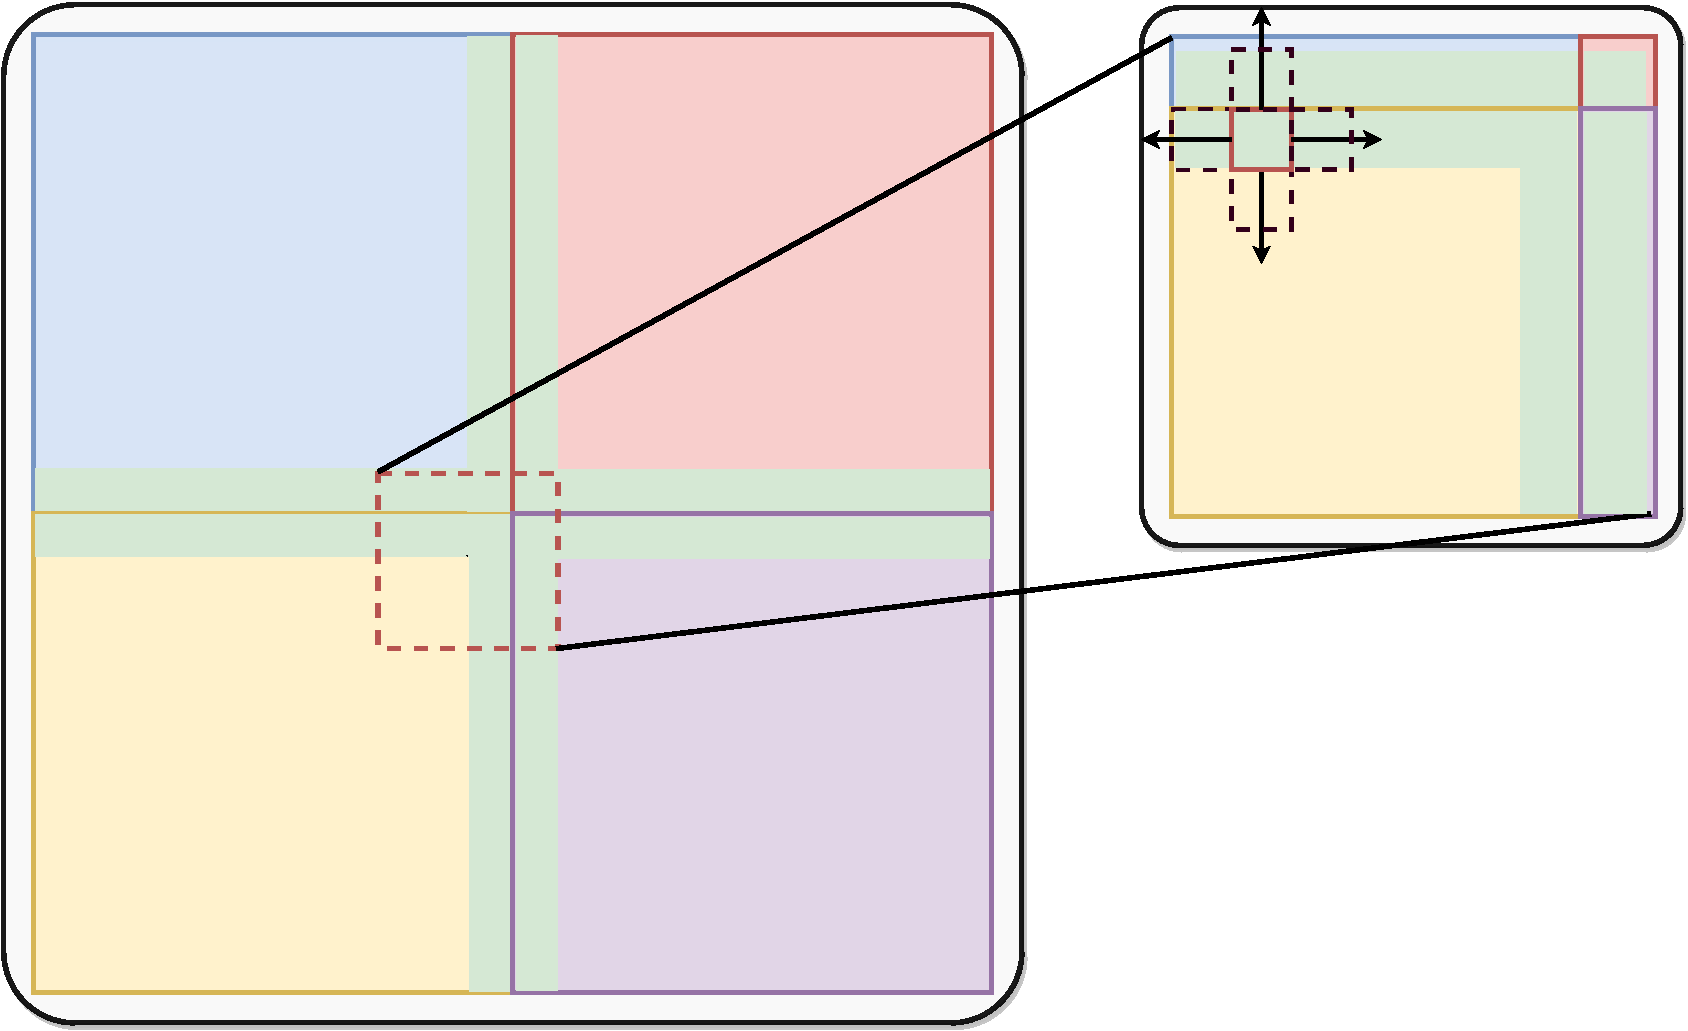
\includegraphics[width=\linewidth]{figs/Stencil.pdf}
  \caption{Distributed stencil kernel}
  \label{fig:stencil-diagram}
\end{figure}

The regions of data depencies that lie on the borders between locales
are known as ghost regions. A parameter known as the stencil radius
determines the width of these ghost regions, and so total amount of data
to be communicated increases linearly with respect to the order of the
matrix. Unlike the transpose kernel, the stencil kernel requires the
communication of only relatively small amounts of data, while providing
a high arithmetic intensity.
